%
% discontinuities.tex -- XXX
%
% (c) 2019 Prof Dr Andreas Mueller
%
\section{Ausbreitung von Unstetigkeiten}
\rhead{Unstetigkeiten}
In der Untersuchung der Lösungen der Wellengleichung zu Beginn
dieses Kapitels wurden Lösungen gefunden, welche durch Verschiebung
einer Anfangswertfunktion $u_0$ entlang der 
Charakteristiken, also der Geraden 
$x\pm at=\operatorname{const}$ erhalten werden können. Ist $u_0$
nicht überall differenziertbar, liefert die Formel immer noch eine
stetige Lösung, die jedoch entlang der Charakteristiken nicht
differenzierbar ist.

Nehmen wir an, $u$ sei mit Ausnahme einer Kurve überall zweimal
stetig differenzierbar.
Auf der Kurve selbst sei nur die erste Ableitung stetig.
Die Kurve teilt den Definitionsbereich in zwei
Bereiche, offenbar ist $u$ in jedem dieser Bereiche eine 
Lösung der Differentialgleichung mit den gleichen Anfangswerten
entlang der Kurve und den gleichen Tangentialebenen.
Da die zweiten Ableitungen aber nicht auch übereinstimmen, muss
die Kurve eine Charakteristik sein.



\begin{satz}
Ist eine Funktion $u$ mit Ausnahme einer Kurve zweimal stetig
differenzierbar, und erfüllt sie die Differentialgleichung
ausserhalb der Kurve, dann ist die Kurve eine Charakteristik.
\end{satz}
Unstetigkeiten können sich also nur entlang von Charakteristiken
ausbreiten.
Die Wellengleichung kann auch zur näherungsweisen
Berechnung der Strömung um ein Überschallflugzeug verwendet werden.
Dabei treten Unstetigkeiten als vom Flugzeug erzeugte Schockwellen
auf, und können als Dichteänderungen mit einer
sogenannten Schlierenaufnahme sichtbar gemacht werden
(Abbildung~\ref{ueberschall2d}).

\begin{figure}
\begin{center}
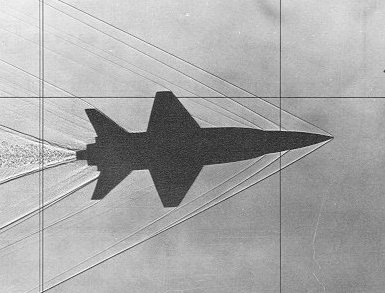
\includegraphics[width=0.8\hsize]{../common/graphics/i-5-1}
\end{center}
\caption{Überschallströmung um ein Überschallflugzeug\label{ueberschall2d}}
\end{figure}

